\newpage
\fancyhf{}
\lhead{Marcel Fuchs}
\rhead{Seite \thepage}
\section{Software - Arduino}
\subsection{Allgemeines}
Für Umsetzung der automatischen Steuerung des Systems wurde, wie bereits erläutert
auf ein Arduino Mikrocontrollerboard gesetzt. Die Programmierung erfolgt über den
bordeigenen Bootloader wodurch kein externer Programmer oder Debugger nötig ist. Des
Weiteren wurde das gesamte Softwareprojekt in der Arduinoeigenen IDE erstellt und editiert.
\subsection{Objektorientierung}
Da das Bewässerungssystem für mehrere Pflanzen geeignet sein soll und man somit
mehrere Aktoren mit denselben Funktionen hat ist es sinnvoll diesen Teil des Software
Projektes Objektorientiert zu gestalten. Die Objektorientierung bietet außerdem den
Vorteil ohne viel Aufwand weitere Pflanzen mit dem System zu bewässern.
\begin{figure}[ht]
    \centering
    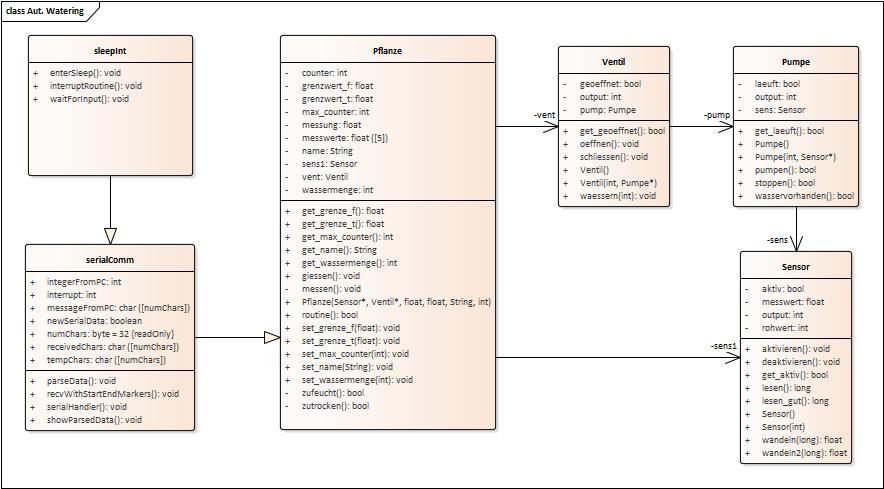
\includegraphics[width=\textwidth]{marcel/AutWatering}
    \caption{Klassendiagramm des Programms auf dem Arduino}
    \label{arduinoklassen}
\end{figure}

So gibt es für jede zu bewässernde Pflanze ein Objekt der Klasse Pflanze. Wie in
Abbildung \ref{arduinoklassen} zu sehen beinhaltet diese Informationen zu allen wichtigen Kenndaten.
So werden ihr Feuchtegrenzwerte, die Wassermenge pro Wässerung, ein Name und die
übliche Zeit zwischen zwei Wässerungen zugewiesen. Außerdem werden das zugehörige
Ventil und der passende Sensor referenziert. Um diese Attribute auch während des
Programmablaufes ändern oder auslesen zu können gibt es diverse „get-“ und „set-“
Funktionen.  Die Datenverarbeitung und Signalerzeugung wird von den restlichen
Funktionen übernommen.
Für den angesprochenen Sensor und Ventil ist ebenfalls je eine Klasse implementiert.
Entscheidend sind hier die Attribute In- bzw. Output. Diese verweisen auf je einen
digitalen GPIO Pin des Arduino Boards. An diesen ist die jeweilige Steuerelektronik
angeschlossen, sodass man über diese Ports das Ventil steuern und den Sensorwert
auslesen kann. Die Funktionen übernehmen wieder den Teil der Datenverarbeitung und
Singalerzeugung. Eine letzte Klasse stellt die Pumpe dar. Von dieser Klasse wird nur
ein Objekt erzeugt, das von jedem Ventilobjekt referenziert wird. Eine kurze
Beschreibung der Funktionen finden sie in der folgenden Tabelle:
\hbadness=10001
\begin{tabular}{|l|p{0.55\textwidth}|}
    \hline
    Name der Funktion &	Funktionsbeschreibung\\ \hline
    Pumpe::pumpen() &	Setzt den Pin High an dem die Pumpe angeschlossen ist, wenn Wasser vorhanden ist.\\ \hline
    Pumpe::stoppen() &	Setzt den Pin Low an dem die Pumpe angeschlossen sit.\\ \hline
    Pumpe::wasservorhanden() &	True: Wenn Wasserstandsensor $< 250kHz$ liefert\\ \hline
    Ventil::oeffnen() &	Setzt Ventil-Pin high\\ \hline
    Ventil::schliessen() &	Setzt Ventil-Pin low\\ \hline
    Ventil::waessern(int dauer) & Startet Pumpe; Öffnet nach fester Verzögerung Ventil; Nach gegebener Dauer wird Ventil und Pumpe geschlossen.\\ \hline
    Pflanze::giessen() &	Pflanze wird gegossen (Ventil::waessern) und Zähler zurückgesetzt.\\ \hline
    Pflanze::zufeucht() &	Basierend auf aktueller und letzten Messungen wird entschieden, ob die Pflanze zu feucht ist.\\ \hline
    Pflanze::zutrocken() &	Basierend auf aktueller und letzten Messungen wird entschieden, ob die Pflanze zu trocken ist.\\ \hline
    Pflanze::routine() &	Aktuelle Feuchte wird gemessen, gespeichert und aufgrund des Wässerungsalgorithmus entschieden, ob die Pflanze nun gegossen wird\\ \hline
    Sensor::lesen() &	Sensor ließt die Frequenz an den zugewiesenen Inputport\\ \hline
    Sensor::wandeln() &	Die gelesene Freuqenz wird in einen prozentualen Feuchtewert gewandelt\\ \hline
\end{tabular}


\newpage
\subsection{Auslesen der Sensoren}
\begin{lstlisting}[caption=Codeabschnitt zum Auslesen]
    for  (int  i  =  0;  i  <  100;  i++)
    {
        pulseHigh  =  pulseIn(this->input,  HIGH);
        pulseLow  =  pulseIn(this->input,  LOW);
        pulseTotal  +=  pulseHigh  +  pulseLow;
    }
    frequency  =  (1.0  /  (pulseTotal/100))*1000000.0;
\end{lstlisting}
Die Feuchtigkeitssensoren liefern an ihren Ausgängen eine sich ändernde
Frequenz. Aus diesen Grund muss das Arduino Programm eine Möglichkeit
haben Frequenzen an einen Eingang zu ermitteln. Dies wird mit dem oben
gezeigten Codeabschnitt bewerkstelligt. Die Standard Arduinofunktion
„pulseIn()“ zählt die Zeit (in $\mu s$), wie lange ein Zustand an
einen Input-Pin anliegt. Das heißt in Zeile 3 wird der Variable
„pulseHigh“ die Zeit zugewiesen in der der Input Pin dieses Sensors
high war. Zusammen mit der Zeit in der der Zustand low anlag
ergibt sich eine Periodendauer. Um Fehler in der Messung der Zeiten
zu verringern wird hundert Mal hintereinander gemessen. In Zeile 7
wird dann die gesamte Messung in eine Frequenz umgerechnet.
\begin{center}
    $f=\frac{1}{t}$
\end{center}
Faktor $10^6$ für die Umrechnung $\mu s$ in $s$.
Divisor $100$ für den Durchschnitt aller Messungen.


\subsection{Kommunikation und Energiesparmodus}
In Abbildung \ref{arduinoklassen} ebenfalls dargestellt sind die Funktionen,
welche für die Kommunikation mit dem zweiten Mikrocontrollerboard nötig sind.
Des Weiteren sind die Funktionen, welche den Stromsparmodus des Arduino
starten, aufgelistet. In der „enterSleep()“ wird zunächst ein externer
Interrupt an den digitalen Pin aktiviert, welcher durch das ESP-Board
ausgelöst werden kann. Danach werden durch Funktionen, welche aus der
AVR „Sleep“ \footnote{https://www.nongnu.org/avr-libc/user-manual/group\_\_avr\_\_power.html}
und „Power“ \footnote{https://www.nongnu.org/avr-libc/user-manual/group\_\_avr\_\_sleep.html}  Bibliothek stammen, alle unwesentlichen
Teile des Arduino abgeschaltet.
Sobald nun ein Interrupt am Arduino
registriert wird, starten diese Teile wieder und die Funktion
„waitForInput()“ wird aufgerufen.
Diese Funktion erwartet nun vom ESP eine Nachricht am serielen Interface. Diese Nachricht
teilt dem Programm mit, welche Aktion als nächstes ausgeführt werden muss. Aus diesem
Grund ist des nötig die Nachrichten von fehlerhaften zu unterscheiden. Die Zeichen „$<$“ und „$>$“
markierten den Anfang und Ende eines solchen Befehls. Die gesamte Syntax eines gesamten Befehls
lautet deswegen: $<$Objekt,Nummer$>$. Folgende Objekte und Befehlsnummer gibt es:
\newline


\begin{tabular}{|l|c|p{0.65\textwidth}|}
    \hline
    Objekt & Nummern & Bedeutung \\ \hline
    Timer & - & Timerinterrupt, Routine jeder Pflanze wird aufgerufen. \\ \hline
    PlantN & 0-9 & 0-4: Wassermenge der Pflanze „N“ wirde geändert.\newline 5: Pflanze „N“ wird sofort gegossen. \newline 6-9: Üblicher Wässerungsrythmus wird geändert.\\ \hline
    Empty & 0,1	& 0: Wasser vorhanden.\newline 1: Kein Wasser vorhanden.\\ \hline
\end{tabular}\label{arduinokomm}

\newpage
\subsection{Bewässerungsalgorithmus}
\begin{wrapfigure}{l}{0.3\textwidth}
    \caption{\\Algorithmus}
    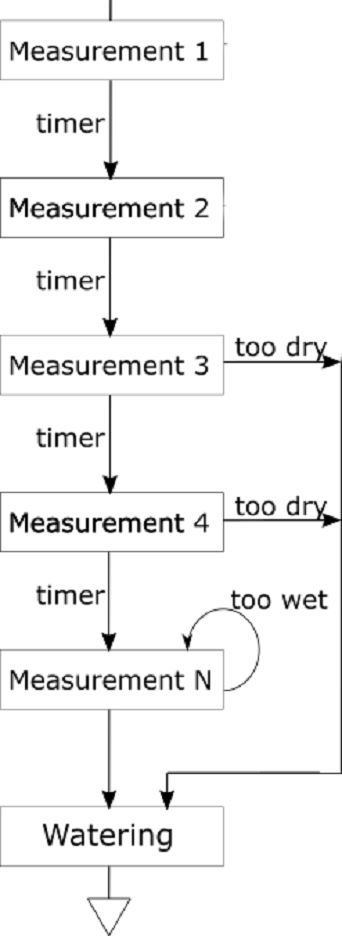
\includegraphics[width=0.3\textwidth]{marcel/algo}
    \label{arduinoalgo}
\end{wrapfigure}
In Abbildung \ref{arduinoalgo} ist der verwendete Bewässerungs-algorithmus zu sehen.
Nachdem das ESP-Programm einen Timerinterrupt an den Arduino gesendet hat,
startet dieser eine Messung an jeder Pflanze. Dabei wird auch ein Zähler
hochgesetzt. Sobald dieser einen einstellbaren Maximalwert erreicht wird
die Pflanze gegossen. Bei einen 8 Stunden Messintervall sind folgende
Bewässerungsrhythmen einstellbar: 1 Tag, 2 Tage, 7 Tage und 10 Tage.
Neben dem zeitbasierten System wird auch noch die Feuchtigkeit im Boden
der Pflanze einbezogen. Die letzten Messwerte der Pflanze werden gespeichert.
Wurde seit zwei Messungen nicht mehr gegossen, werden die letzten Messwerte
mit den voreingestellten Messwerten der Pflanze verglichen. Waren die
Messwerte unter der Trockengrenze wird eine verfrühte Bewässerung ausgeführt
und dabei der Zähler zurückgesetzt. Wird der maximale Zählerwert erreicht
werden die Messwerte mit dem Feuchtegrenzwert verglichen, sind sie zu hoch
und die Bewässerung ausgesetzt. Der Zähler wird dabei nicht zurückgesetzt,
sodass nach einen weiteren Timerinterrupt die Feuchte erneut getestet wird
und ggf. dann gegossen wird.

\newpage
\subsection{Programmablauf}
\begin{figure}
    \centering
    \includegraphics[width=0.9\textwidth]{marcel/ablauf}
    \caption{Ablauf des Programms}
\end{figure}
Nach dem Start des Arduinos wird zunächst das Setup durchlaufen, Alle Objekte mit
Startwerten initialisiert und das Hardwaresetup gemacht. Danach wird der Arduino
in den Sleep bzw. Energiesparmodus gebracht.  Sobald nun ein Interrupt des ESP an
den Arduino gesendet wird, erwacht dieser und erwartet einen Befehl am seriellen
Interface. Dieser wird ebenfalls vom ESP gesendet, um dann ausgewertet werden zu
können. Beinhaltet die Nachricht einen Befehl zum Ändern eines Wertes einer Pflanze,
wird dieser Wert geändert und der Arduino wieder in den Sparmodus versetzt. Handelt
es sich bei der Nachricht aber um einen Timerinterrupt, wird bei jeder Pflanze die
Routine gestartet. Wie bereits beschrieben, wird zunächst der zugehörige
Feuchtigkeitssensor ausgelesen, der Messungszähler erhöht und die vorliegende
Feuchtigkeit ausgewertet. Danach wird je nach Ergebnis der Auswertung der Sleep
Modus erneut gestartet oder mit der Bewässerung gestartet. Das Softwareobjekt
Pflanze schickt ein Signal an das zugehörige Ventil welches ein weiteres Signal
an die Pumpe schickt. Ist der Bewässerungsvorgang abgeschlossen, wird der Zähler
zurückgesetzt und der Energiesparmodus wird gestartet. 
